\chapter{Konzeption und Aufbau des Prototyps}
% In diesem Kapitel wird die Konzeption des Prototyps vorgestellt.
% % Sie enthält zunächst das methodische Vorgehen des Abschnitts, im Anschluss folgt eine Analyse der Spiele, die im Fokus der Arbeit stehen und aus welchen Aspekte in die Konzeption eingeflossen sind. Der Hauptteil der Konzeption umfassen das Game-Design des Prototyps.

Nachdem durch die Literaturrecherche in Kapitel \ref{sec:related-works} wichtige Funktionalitäten im Design identifiziert werden konnten und vergleichbare Spiele in Kapitel \ref{sec:analysis} auf ihr Game- und Rätseldesign analysiert wurden, kann aus den Ergebnissen \say{Connecting-Minds} nun vollständig konzipiert werden. \cite{krekhov_puzzles_2021} beschreibt eine Taxonomie für analoge und digitale Escape-Room Spiele, die ebenfalls in die Konzeption des Spiels hineinfließen. Außerdem werden sinnvolle Design-Patterns für kooperative Spiele aus den Arbeiten von \cite{guimaraes_rocha_game_2008} und \cite{seif_el-nasr_understanding_2010} ausgewählt und integriert.

Die Konzeption dieses Spiels folgt einem methodischen Vorgehen: Zunächst wird die übergeordnete Designvision und Zielsetzung erläutert. Anschließend dient das \ac{MDA}-Framework (vgl. \cite{hunicke_mda_2004}) als zentrales Analyse- und Strukturierungsmittel, um das Spielerlebnis gezielt zu gestalten. Auf Basis des \ac{MDA}-Frameworks werden die grundlegenden Spielmechaniken, Rollenverteilungen und dynamischen Abläufe beschrieben.

\section{Designziele und Zielgruppe}
\say{Connecting-Minds} verfolgt das Ziel, kooperative Kommunikation unter ungleichen Perspektiven in einem Escape-Room-ähnlichen Szenario zu verbessern. Dabei existieren zwei verschiedene Rollen - Player und Watcher - die gemeinsam die Rätsel lösen und Hindernisse der Spielwelt überwinden müssen. Die Wahrnehmung der Spielwelt und Handlungsmöglichkeiten ist in beiden Anwendungen unterschiedlich, gleichzeitig ergänzt sie sich aber. 

Das Genre des Spiels ist demnach ein kooperatives Adventure-Spiel.

Ziel ist es, durch asymmetrische Informationsverteilung eine Spannung zwischen Orientierung und Vertrauen aufzubauen und gleichzeitig den gemeinsamen Fortschritt in den Mittelpunkt zu stellen.

Die Zielgruppe bleibt dabei identisch zu der, die in der vorangegangenen Ausarbeitung im Modul \emph{Interaktionsdesign} entstanden ist.

Zunächst gibt es da den 19 Jahre alten Steve Works, der Medieninformatik-Student im ersten Semester ist. Er strebt nicht nur nach akademischen Erfolg, sondern auch nach sozialer Interaktion. Er plant gerne Spieleabende und Partys um Kontakte zu knüpfen und um den Spaß am Studieren zu betonen.

Uwe Kaufmann, 64 Jahre alt, ist ein erfahrenere Projektleiter und steht vor der Herausforderung ein neues Team zu formen. Sein Ziel ist es, durch Teambuilding und Motivation eine effektive Zusammenarbeit zu formen.

Anja Gayms, 31 Jahre alt, ist eine introvertierte Zahnarzthelferin und such in \say{Connecting-Minds} nach einer geistigen Herausforderung und einer Möglichkeit, ihre Freundschaften zu stärken.

Die 3 Personae sind in ihrer Gesamtheit in Anhang \ref{} verfügbar.


\section{Narratives und funktionales Grundgerüst}
% [Text nochmal kürzen]
Das Spiel basiert auf einem asymmetrischen Zwei-Rollen-Prinzip, bei dem zwei Spieler zwei unterschiedliche Rollen spielen. Sie müssen gemeinsam in der Spielwelt agieren. Die Spielwelt ist in verschiedene Räume gegliedert, welche modular aufgebaut sind. Durch das Zusammenarbeiten und das gemeinsame Lösen der Rätsel kann ein Spielfortschritt erzielt werden.
% Die beiden Rollen des Spiels werden Player und Watcher genannt. Der Player bewegt sich mit einer Isometrischen Perspektive durch die Spielwelt und kann die Ansicht bei Bedarf auch in die Egoperspektive wechseln. Er befindet sich dabei innerhalb der Spielwelt und interagiert von dort mit ihr.
% Der Watcher befindet sich ebenfalls in einer Isometrischen Ansicht, besitzt allerdings keinen eigenen Avatar in der Spielwelt. Er befindet sich außerhalb der Spielwelt, kann aber dennoch mit der Spielwelt interagieren. Der Watcher kann die Spielwelt in \ac{AR} vor sich platzieren um so um die Spielwelt herum zu gehen, oder sich einzelne Elemente näher anschauen.

Das Narrativ der Handlung und der Geschichte werden durch Textuelle Hinweise und Geschichten sowie dem Aufbau der Umgebung erzählt. 

% Funktional basiert das Spiel auf dem lösen von Rätseln und beseitigen von Hindernissen, die nur durch die Kombination beider Rollen lösbar sind.

Die Hintergrundgeschichte des Spiels ist folgende:

Der Protagonist der Handlung sollte in seinem Forschungsinstitut eine Simulation [Simulation zu was noch einbauen] ausprobieren. Allerdings kam es während der Simulation zu einer Anomalie, wodurch sich sein Sein aufgespalten hat. Übrig blieb sein physisches Ich, das in seinem Forschungsinstitut zurück blieb und sein abgespaltener Geist im Netz der Forschungseinrichtung. Sein aufgeteiltes Ich kann auf eine besondere Weise (vermutlich ausgelöst durch die Anomalie der Simulation) miteinander kommunizieren. Gemeinsam versuchen sie nun herauszufinden wer für diese Anomalie verantwortlich ist und wie das physische Ich wieder mit seinem Geist zu einer Person zusammengefügt werden kann.

% Das Genre des Spiels ist demnach ein kooperatives Adventure-Spiel das in einem Low-Poly \ac{Sci-Fi}-Setting spielt.

% [Text zur Spielwelt, wo sich Schauplätze überall befinden ausdenken]
% Zunächst befinden sich die Spieler in einem alten Verlies
Die Spielwelt umfasst dabei zunächst ein altes Kellergewölbe der Forschungseinrichtung, in welcher der Körper des Players gebracht wurde, nachdem die Simulation schief lief. Des weiteren durchläuft der Player, mit seinem Watcher im Gepäck, die Forschungseinrichtung und sucht nach Hinweisen auf einen möglichen Antagonisten. Die Spielwelt wird erweitert durch Außenbereiche um die Forschungseinrichtung herum und geht weiter in die Privathäuser nzw Wohnungen von beteiligten Personen.

\section{Spielkonzeption mithilfe des MDA-Frameworks}
Aus den bisherigen Forschungen zum Thema asymmetrischen kooperativen Spielen und Kommunikation geht hervor, dass die Spielerrollen des Spiels in ihren Funktionen und/ oder ihrer Ansichten eine Abhängigkeit von einender bestehen muss. Diese Abhängigkeit darf nicht zu groß sein, da sonst der Spielfluss gestört werden würde und Frust bei den Spielern entstehen würde. 

Die Analyse der artverwandten Spiele zeigten Inhalte und Funktionalitäten, die in ihrer Form so integriert werden sollten, aber auch zu viel bzw. zu eigenständig sein könnten, wodurch ein kooperatives Verhalten gestört werden kann.

Aus der \say{We were here}-Spielreihe geht hervor, dass die Rätselelemente so gestaltet werden müssen, dass diese für den anderen Mitspieler beschreibbar und verständlich erklärbar sind. Außerdem sollten die Anwendungen eine höhere Dynamik zwischen sich haben, wodurch eine engere Beziehung der Spielerfahrung und der Anwendungen entsteht. 

\say{Tiny Room Stories} zeigt wie einzelne Rätselelemente und freischalten von Hindernissen so zusammenhängen können, dass viele kleine Elemente zu einem großen Ziel führen können. Außerdem bietet es für die Steuerungsmechanik eine Inspirationsquelle. 

\say{The past within} zeigt, dass ein zu hohes Forderungslevel der einzelnen Anwendungen unvorteilhaft für die Förderung der Kommunikation ist. Es führt dazu, dass jeder Spieler auf seine Anwendung fixiert ist, aber seltener ein Gefühl dafür bekommt, wann er seinen Mitspieler benötigt und wann er selbständig Rätsel lösen kann. 

\say{Myrmidon} zeigt auf, wie die einzelnen Anwendungen abhängig zueinander sein können, allerdings fehlt es an einem ausgeglichenem Spielerlebnis. Die beiden Rollen sind so gestaltet, dass der Animator die Stop-Motion Puppe unterstützt und dadurch zu wenig für sich selbst spielt. 

Bei \say{Keep Talking and Nobody Explodes} ist es ähnlich wie bei \say{Myrmidon}, die Spielerrolle der Experten unterstützt hierbei nur den Bombenentschärfer.


% Die Rückschlüsse sind folgende:

% \begin{itemize}
%     \item Aus der \say{We were here}-Spielreihe geht hervor, dass die Rätselelemente so gestaltet werden müssen, dass diese für den anderen Mitspieler beschreibbar und verständlich erklärbar ist.
%     \item Außer
%     % \item 
%     % \item 
%     % \item 
% \end{itemize}

% \subsection{Inhalte aus der Literaturrecherche}
% \subsection{Inhalte aus der Analyse der Spiele}
% \subsection{Inhalt aus der Taxonomie}

\subsection{Mechanics}
Die Mechanischen Elemente des Spiels werden in die zwei jeweiligen Spielerrollen (Player und Watcher) und allgemeingültigen Mechaniken aufgeteilt.

\paragraph{Player}
Der Player steuert entweder über die Maussteuerung (Point \& Click-System) oder über Touchinputs den Avatar in der Spielwelt. Über das Mausrad oder die Zoom-Touch Steuerung kann die Höhe der Kamera zum Avatar verändert werden. Außerdem kann er die Ansicht zwischen der Standard isometrischen Perspektive und einer First-Person-Ansicht wechseln. Das \ac{UI} des Players besitzt eine Toolbar, über die der Avatar bestimmte Interaktionen mit den Weltgegenständen wie das Aufnahmen oder Platzieren vollführen kann. Außerdem kann der Player Gegenstände tragen und diese an den Watcher zurück schicken. Über die First-Person-Ansicht kann der Player ebenfalls Gegenstände platzieren.

Außerdem schaltet der Player neue Gegenstände in der Spielwelt frei, in dem er so nah an sie herangeht, dass er mit ihnen interagieren kann.

\paragraph{Watcher}
Der Watcher hat in seiner \ac{AR}-Anwendung die Spielwelt vor sich platziert und kann im physischen Raum um die Spielwelt herumgehen und auch in die Spielwelt hinein um sich die Welt genauer anzusehen. Seine Aufgaben liegen darin, eine Übersicht über die Spielwelt und alle gesammelten bzw. platzierten Gegenstände zu haben. Er kann alle interagierbaren Gegenstände, die entdeckt und platziert wurden von der Spielwelt entfernen. Die Gegenstände gehen danach wieder in das Inventar über, auf welches nur er Zugriff hat. Er kann bestimmte Gegenstände in der Spielwelt über einen Touch-Input platzieren oder andere Gegenstände an den Player schicken, welche der Player dann trägt. 

Im weiteren Verlauf des Spiels kann der Watcher Gegenstände nicht nur platzieren oder entfernen, sondern auch in der Größe skallieren oder drehen.

\paragraph{Weltregeln}
Leichte Gegenstände können vom Player getragen und aufgenommen werden. Diese Gegenstände kann der Player in der Spielwelt über die Interaktions-Leiste oder in der First-Person platzieren. 

Schwere Gegenstände können nur vom Watcher platziert oder skaliert werden. Der Player kann jedoch über seine Interaktionen mit ihnen interagieren. Beide Arten von Gegenständen können, sobald sie entdeckt und in der Spielwelt platziert wurden vom Watcher wieder entfernt werden.

Es existieren zudem Hinweise in Schrift- und Bildform, welche vom Player entdeckt und an den Watcher gesendet werden können. Sie gälten als Ergänzung zum Environmental Rätseldesign.

\subsection{Dynamics}
Die aus den Mechaniken folgenden Dynamiken beziehen sich auf die Asymmetrie in der Perspektive und den Informationen, die beide Spielerrollen haben und erhalten. Außerdem entsteht dadurch eine Kombination aus den gegebenen Informationen, um daraus die richtigen Ansätze für Lösungen zu finden. 
Es entsteht eine Kombination und Koordination der Fähigkeiten der beiden Rollen, durch welche erst das Lösen der Hindernisse ermöglicht wird.

Durch die AR-Anwendung des Watchers entsteht eine neue räumliche Orientierung, da die Spielwelt in die physische Welt eingebettet wird.


\subsection{Aesthetics}
Die durch das Spiel angesprochenen ästhetischen Eigenschaften sind Challenge, Fellowship und Expression. Das Spiel soll logisches Denken, die Kommunikation und die Koordination der Spielteilnehmer anregen. Außerdem soll durch die enge Verknüpfung der Rollen eine enge Zusammenarbeit entstehen, durch welche ein Gemeinschaftsgefühl aufgebaut werden soll. Durch die Kommunikation sollen die Spieler auch sich selbst näher kennenlernen und herausfinden wie man mit sich selbst am besten umgeht.

Untergeordnet steht das Narrativ des Spiels als Stütze für die Sinnhaftigkeit der Herausforderungen, die bewältigt werden müssen.


\section{Spielabläufe}
Die Spielabläufe des Spiels werden in zwei unterschiedliche Abschnitte unterteilt. Es gibt einen übergeordneten Ablauf für das gesamte Spiel und einen für jeden einzelnen Abschnitt.

\subsection{Ablauf des Spiels}
\begin{figure}[ht]
\centering
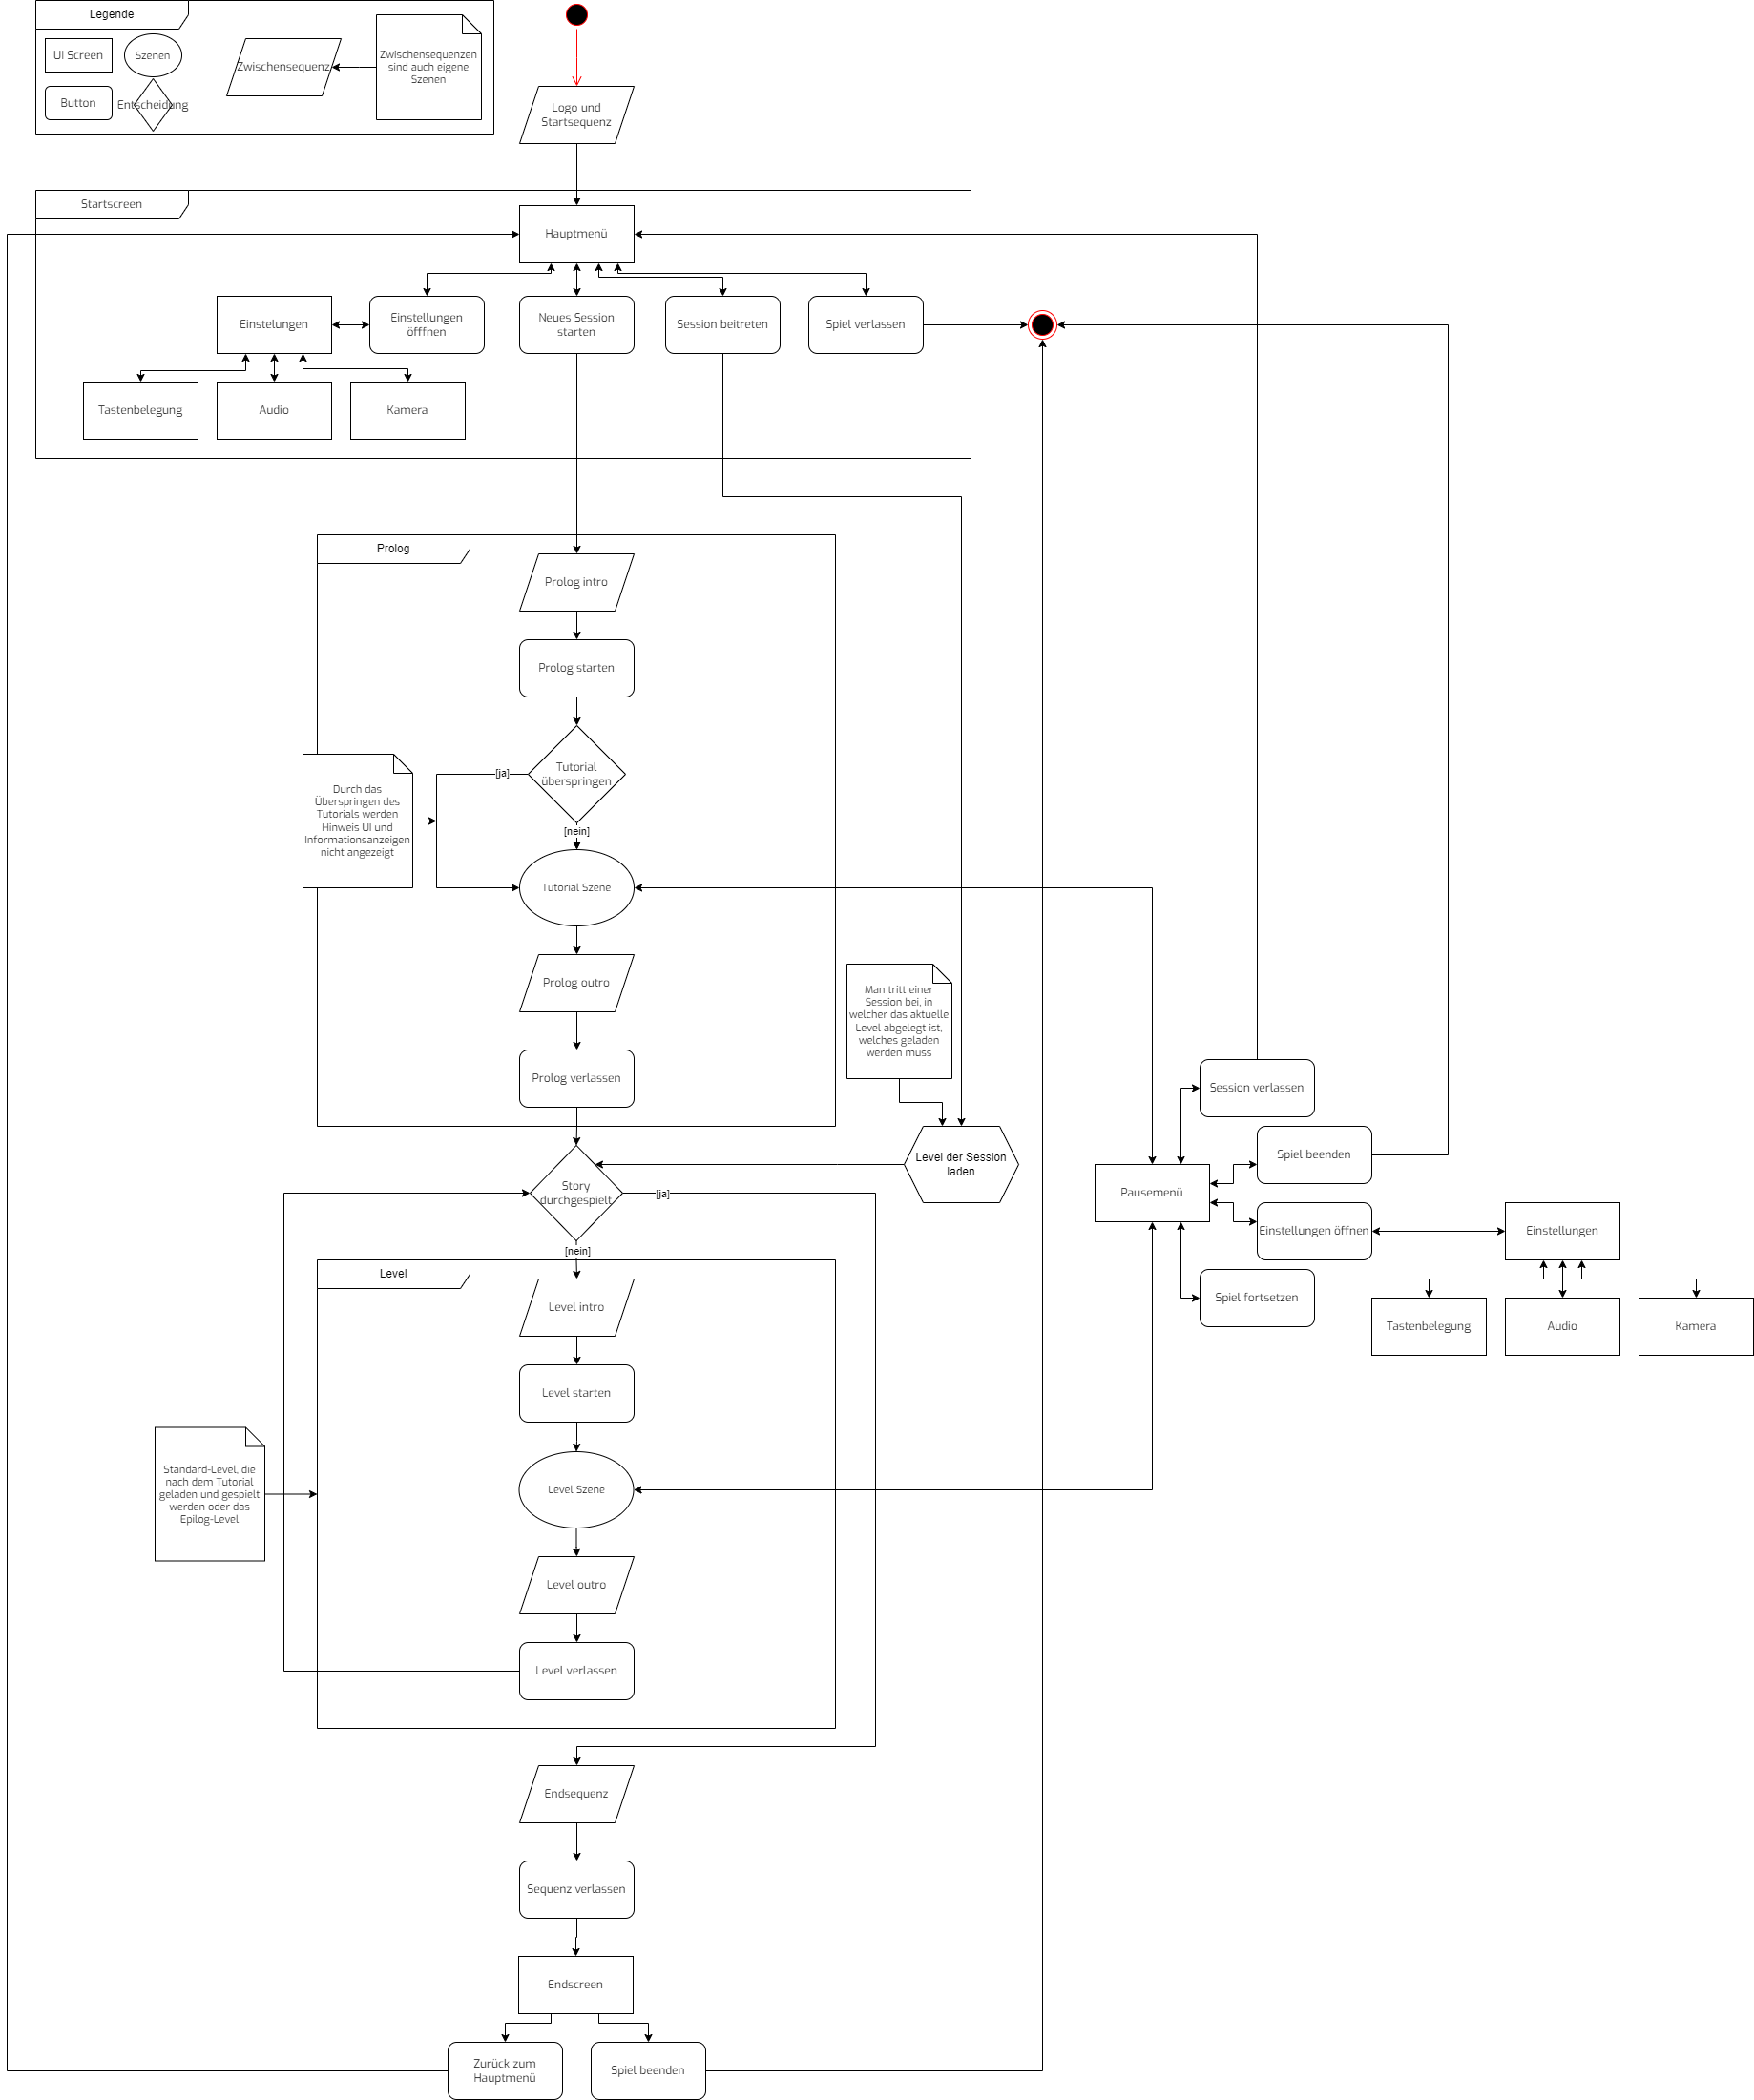
\includegraphics[width=1\linewidth]{content/pictures/GameLoop-Player.drawio.png}
\caption{Aktivitätsdiagramm des gesamten Spiels aus Player Sicht, (Quelle: eigene Darstellung), (in groß im Anhang \ref{})}
\label{fig:game-loop-player}
\end{figure}

\begin{figure}[ht]
\centering
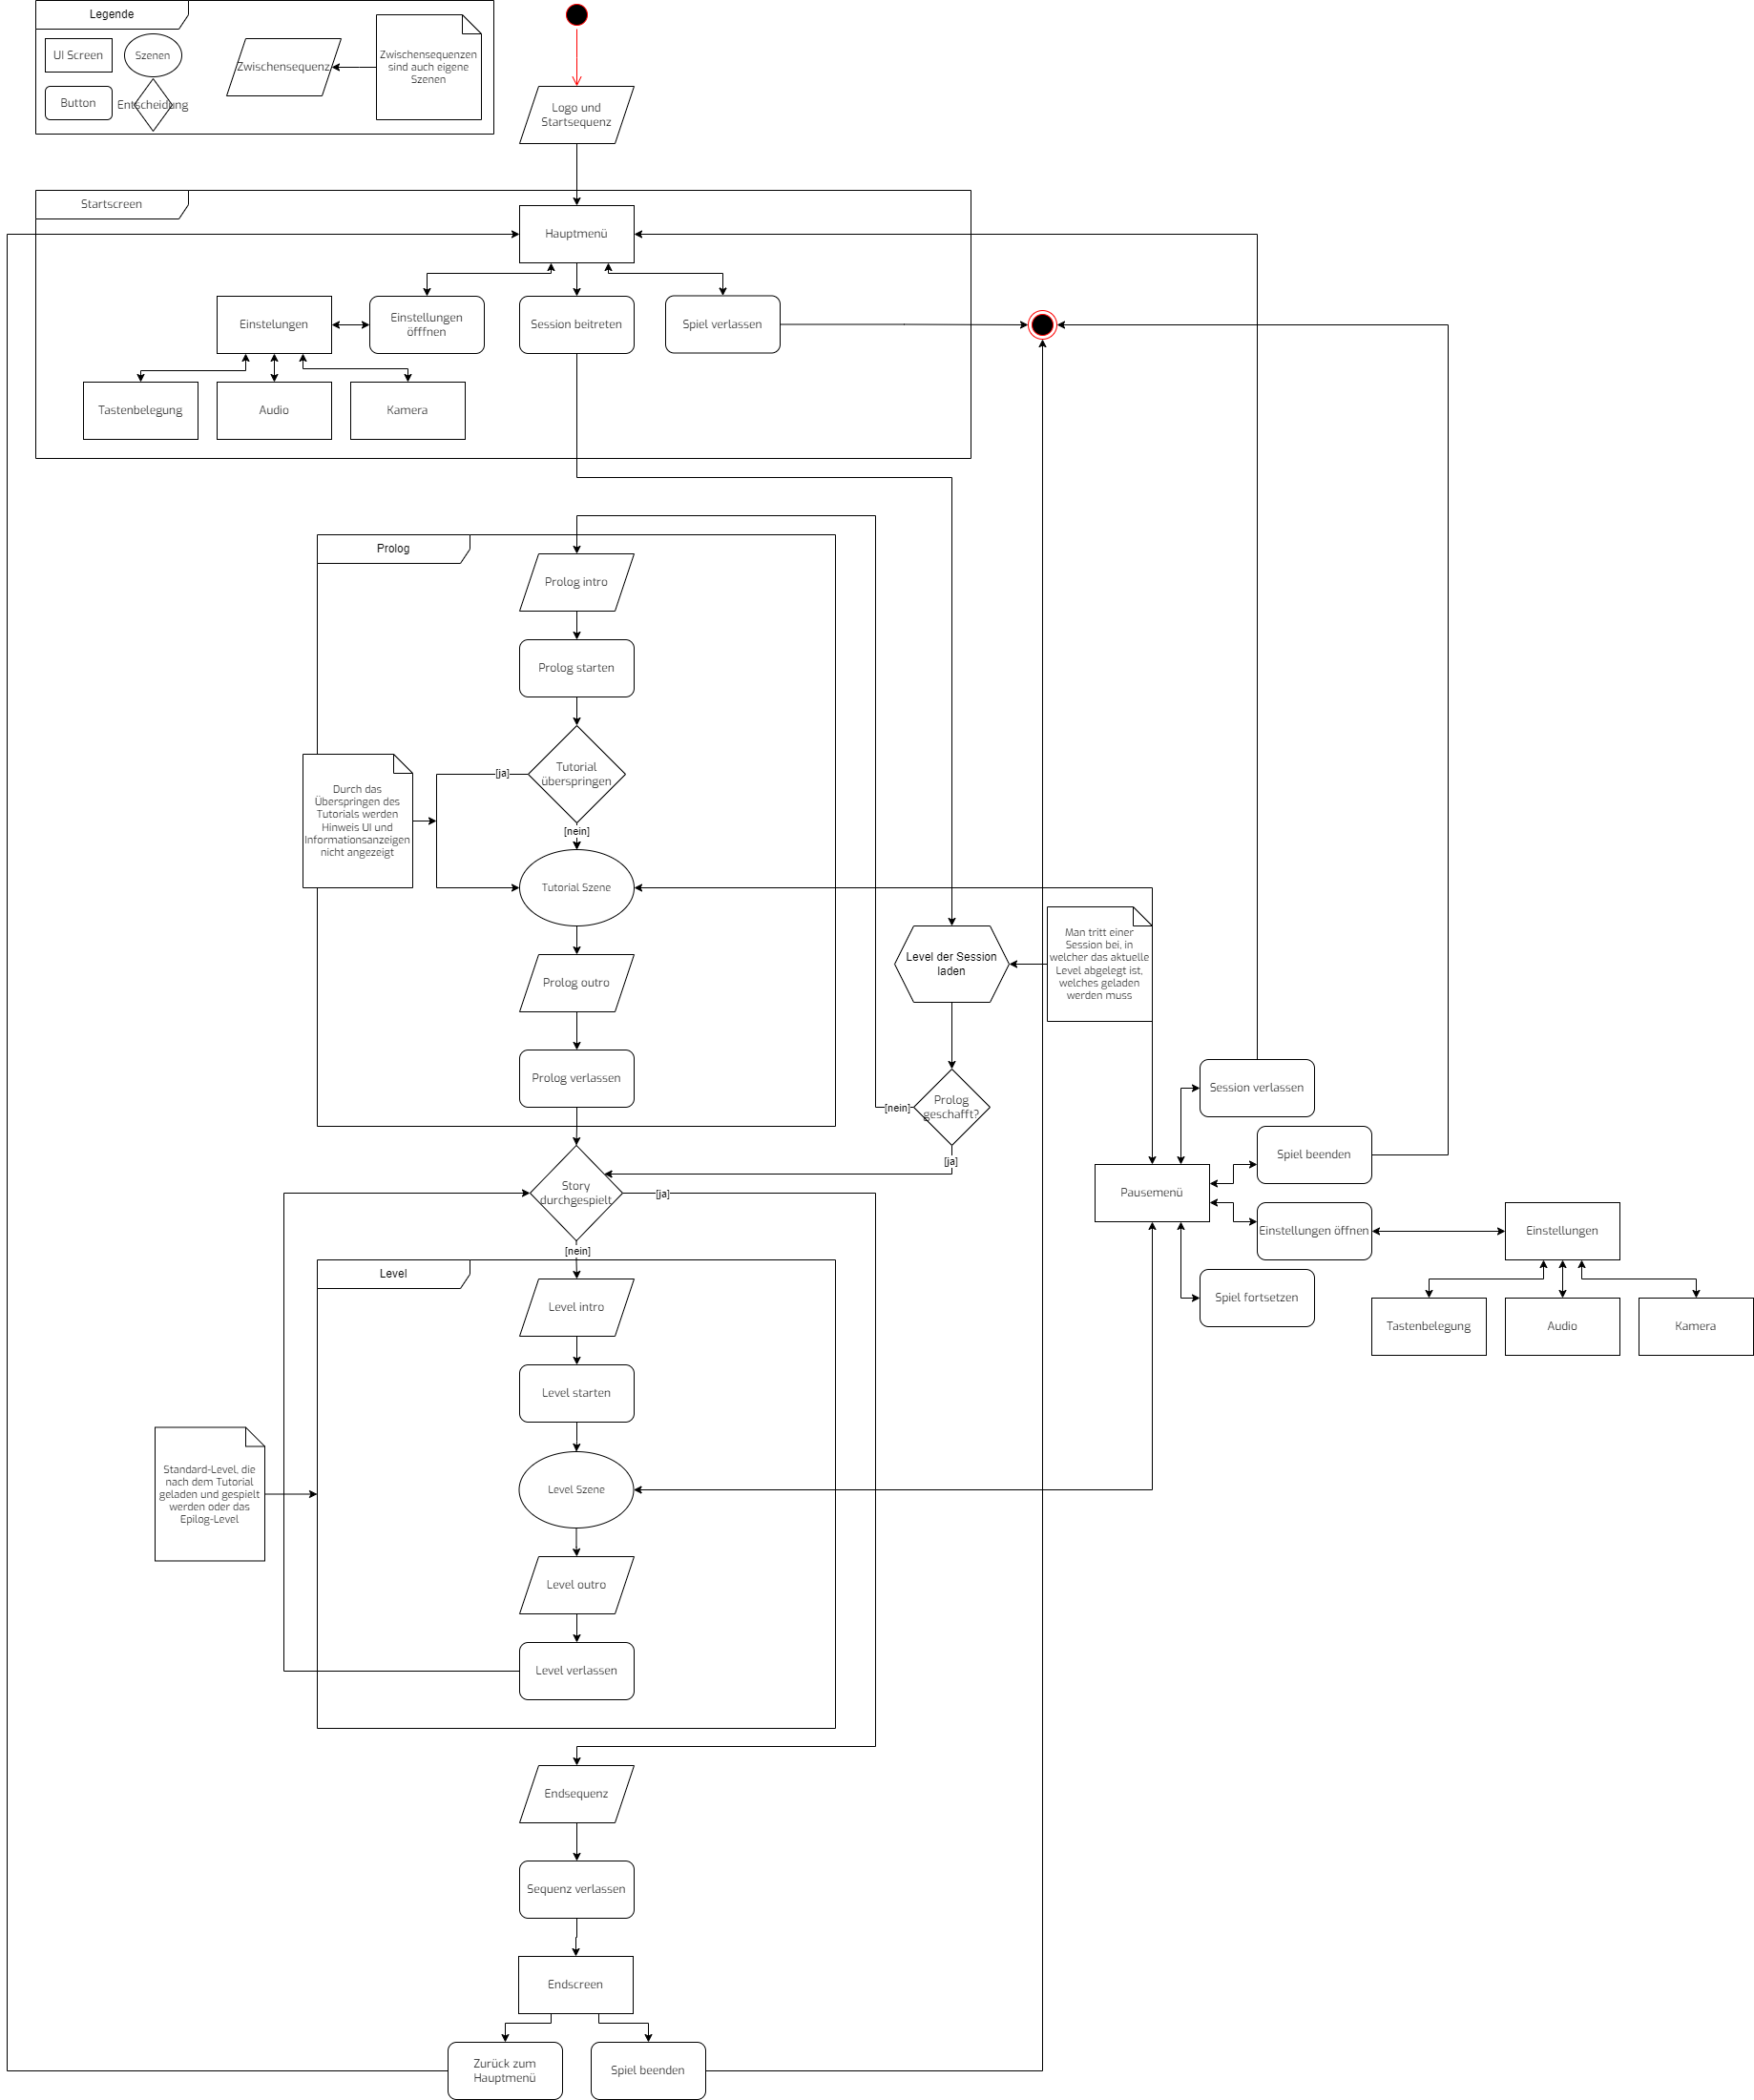
\includegraphics[width=1\linewidth]{content/pictures/GameLoop-Watcher.drawio.png}
\caption{Aktivitätsdiagramm des gesamten Spiels aus Watcher Sicht, (Quelle: eigene Darstellung), (in groß im Anhang \ref{})}
\label{fig:game-loop-watcher}
\end{figure}

Die Abläufe des Spiels sind bei den Anwendungen des Watchers und Players nahezu identisch. Es gibt allerdings einen Unterschied, der im folgenden bei der Beschreibung der Abläufe erklärt wird.
Abbildung \ref{fig:game-loop-player} zeigt das Aktivitätsdiagramm der Player-Anwendung. Sobald das Spiel geladen hat, öffnet sich das Startmenü über das der Player in die Einstellungen gehen, eine neue Session starten, einer existierenden Session beitreten oder das Spiel wieder beenden kann. Über die Einstellungen kann der Player die Tasten bzw. Touchbelegung einstellen, sowie Audio und Kameraeinstellungen ändern. Sobald der Player eine neue Session startet, öffnet sich die Prolog-Szene in der es ein kleines Tutorial zu den Regeln des Spiels und den Steuerungen gibt. 

Über die Tutorial-Inhalte erfährt der Spieler Informationen zu Interaktionsmöglichkeiten mit Gegenständen in der Welt. Sobald sich der Avatar des Players nahe an Gegenstände bewegt, die ein Tooltip haben, kann der Player über eine Leiste mit Interaktionen im UI mit den Gegenständen interagieren. Darunter fällt z. B. das bestätigen einer Taste bei einem Computer oder aber das Aufnehmen und Tragen von Gegenständen.

Es gibt für das Tutorial die Option erklärende Inhalte zu überspringen, da es sein kann, dass der Spieler das Spiel bereits einmal gespielt hat und die Inhalte nicht erneut lesen muss. Innerhalb des Spielszene kann der Player in ein Pausenmenü schalten, worüber er Einstellungen ändern, das Spiel beenden oder die Session verlassen kann. Außerdem kann er das Spiel auch wieder fortsetzen und weiterspielen. Verlässt der Spieler die Session, so lädt erneut der Startbildschirm und kann entweder der verlassenen Session neu beitreten oder eine neue Session starten.

Nach Abschließen des Tutorials wird die nächste Szene geladen, welche in der bestehenden Session gespeichert wird. Sobald der Player nun die Session verlässt und erneut beitritt so lädt die Szene des abgespeicherten Levels. Dieser Kreislauf endet erst, sobald der letzte Spielabschnitt erreicht und die Geschichte beendet wurde. Über den Endscreen gelangt der Player erneut zum Hauptmenü, worüber eine neue Session gestartet werden kann. Das Beitreten der Session des beendeten Spiels führt dazu, dass der Player wieder im Endscreen landet und zurück ins Hauptmenü gelangt oder das Spiel beenden kann.

Bei der Anwendung des Watchers gibt es einen Unterschied zu der des Players. In Abbildung \ref{fig:game-loop-watcher} ist zu sehen, dass der Watcher nach Laden und Starten des Spiels keine Session starten sondern lediglich einer Beitreten kann. Der Watcher ist so konzipiert, dass er nicht der aktive Teilnehmer, sondern ein unterstützender Teilnehmer des Spiels ist. Außerdem erhält der Watcher im Prolog für seine Aufgaben und seine \ac{UI}s entsprechende Informationen. Er erhält Informationen darüber, dass er über das Menü \say{Platzieren} Gegenstände in die Spielwelt platzieren kann und diese über angezeigt Tooltip der Gegenstände auch wieder entfernen kann. Außerdem kann er über das Menü \say{Preview} Gegenstände an den Player senden, welche dieser trägt. Das gilt für jede Gegenstände die der Player trägt. Findet er einen Gegenstand und trägt ihn, so kann der Watcher ihn ebenfalls entfernen. Entdeckte Gegenstände werden wie platzierte Gegenstände in der Welt angezeigt.

Der restliche Spielablauf des Watchers ist identisch zu dem des Players.

\subsection{Ablauf des Levels}
Wie beim Ablauf des Spiels gibt es auch beim Levelablauf zwischen dem Player und Watcher kleine Unterscheidungen, die in der folgenden Erklärung aufgezeigt werden.

\subsection{Ablauf des Spiels}
\begin{figure}[ht]
\centering
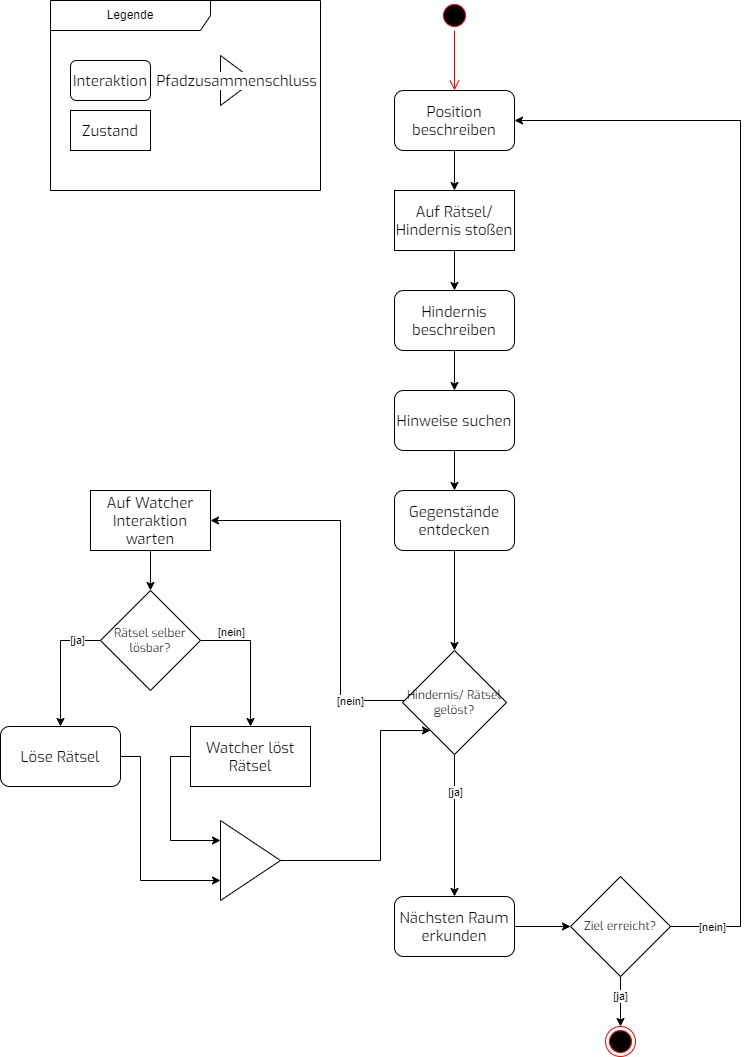
\includegraphics[width=1\linewidth]{content/pictures/LevelLoop-Player.drawio.png}
\caption{Aktivitätsdiagramm des Levels aus Player Sicht, (Quelle: eigene Darstellung)}
\label{fig:level-loop-player}
\end{figure}

\begin{figure}[ht]
\centering
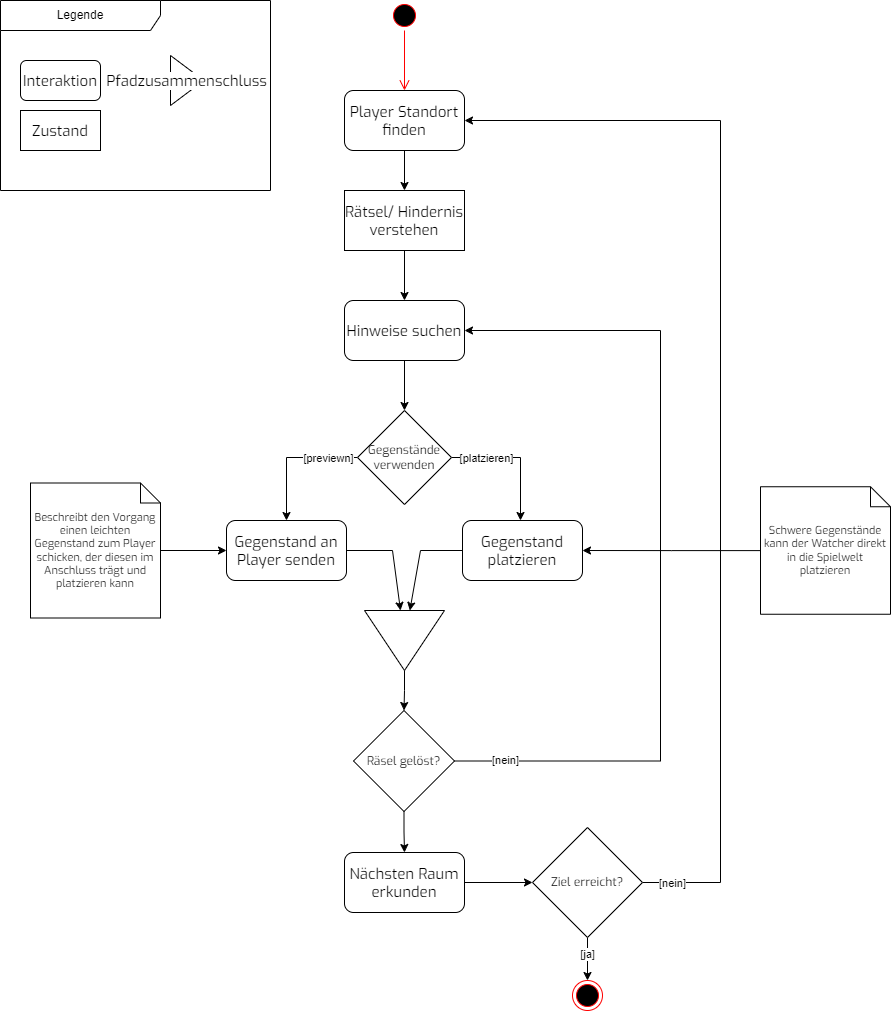
\includegraphics[width=1\linewidth]{content/pictures/LevelLoop-Watcher.drawio.png}
\caption{Aktivitätsdiagramm des Levels aus Watcher Sicht, (Quelle: eigene Darstellung)}
\label{fig:level-loop-watcher}
\end{figure}

Abbildung \ref{fig:level-loop-player} zeigt das Aktivitätsdiagramm des Players innerhalb der Spielszene. Sobald die Szene geladen hat, befindet sicher der Avatar des Spielers irgendwo in der Spielwelt. Da der Watcher den Avatar des Players nicht sehen kann, muss der Player seine Position beschreiben. Entweder nachdem der Player seine Position beschrieben hat oder währenddessen kann er sich in der Welt umsehen und stößt auf erste Rätsel oder Hindernisse. Ist dem so, so muss er seinem Watcher beschreiben um was für ein Rätsel oder Hindernis es sich handelt. In der Spielwelt befinden sich passende Lösungsgegenstände zu den Rätseln, die vom Player entdeckt werden können. Haben der Player und der Watcher das Rätsel gelöst so kann es sein, dass der Player darauf warten muss, dass der Watcher die richtigen Gegenstände in die Spielwelt platziert, damit sie weiter voran kommen oder aber der Watcher muss dem Player die richtigen Gegenstände schicken, damit dieser die Gegenstände an entsprechende Slots oder Stellen platzieren muss. Sobald ein Rätsel gelöst oder Hindernis beseitigt wurde, kommen sie weiter in der Spielwelt voran und müssen die nächsten Räume untersuchen. 

Beim Watcher, dessen Aktivitätsdiagramm in Abbildung \ref{fig:level-loop-watcher} zu sehen ist, verhält es sich ein wenig anders als beim Player. Der Watcher muss zunächst den Standort des Players durch seine Beschreibungen lokalisieren. Während der Lokalisierung und im Anschluss darauf kann er Hindernisse oder Rätsel erkennen und diese dem Player Beschreiben. Außerdem kann er sich bereits Gedanken zu Rätseln und Hindernissen machen, die der Player bereits entdeckt hat. Gemeinsam suchen sie getrennt nach Hinweisen und versuchen Lösungen zu finden. Das Lösen der Rätsel funktioniert aus der Sicht des Watchers ein wenig anders, da er dafür zuständig ist, die jeweilig richtigen Gegenstände zu platzieren und/ oder dem Player zu senden. Sobald alles Rätsel in Koordination gelöst wurden und neue Räume zugänglich sind, fängt der Ablauf von neuem an.

\section{Relation der Anwendungen}
In der bisherigen Konzeption wurde bislang nur über die verschiedenen Rollen gesprochen, aber nicht wie viele Nutzer pro Rolle es pro Session des Spiels sein können. In der Entstehung des Projekts in der vorangegangenen Ausarbeitung war geplant, dass es pro Session immer einen Player geben muss. Außerdem können es immer mehr als einen Watcher geben. Es sollte also diese Regel gälten: $1\ldots n$ \quad wobei $n \geq 1$. In einer Referenz-Bachelorarbeit wurde ein ähnlicher Prototyp konzipiert, bei der in der Auswertung das Feedback gegeben wurde, dass sich mehrere Teilnehmer in der Rolle der \say{Smartphone}-Nutzer (Navigator) nicht zielführend sind (vgl. \cite[S. 34]{lotz_konzeption_2021}). Aus diesem Grund und der Tatsache, dass die Rolle des Watchers eine ähnliche des Navigators ist, sollten pro Session jeweils ein Player mit einem Watcher gemeinsam spielen. Darüber hinaus erforschte die Arbeit von \cite[S. 197:22]{bautista_isaza_understanding_2024} den Einfluss der Gruppengrößen auf das Engagement und die Arbeitsbelastung in einem Handheld-\ac{MR} und \ac{VR} Szenario und kam zu dem Schluss, dass kleinere Gruppen der Effekt des Engagements größer ist. Daraus ergibt sich die Regel $1\ldots1$, durch welche ein Player und ein Watcher in einer Session zusammenspielen.
% \section{Levelablauf}

\section{Konzipiertes Tutorial}
Für diesen Prototyp wurde ein kleines Tutorial konzipiert, durch welchen der Watcher und der Spiele die grundlegenden Mechaniken und Funktionen des Spielkonzepts erlernen können. Aus dem Grund des Umfangs der Umsetzungen, wurden in den Probandentests die einzelnen Funktionen und Steuerungselemente erklärt, die in einem finalen Build im Spiel enthalten sein werden.

Das Tutorial wurde in verschiedene Abschnitte unterteilt, welche sich in einzelne Räume gliedern. Die einzelnen Abschnitte und ihre Räume werden nun vorgestellt.
\subsection{Abschnitt 1: Der Start}

\begin{figure}[ht]
\centering
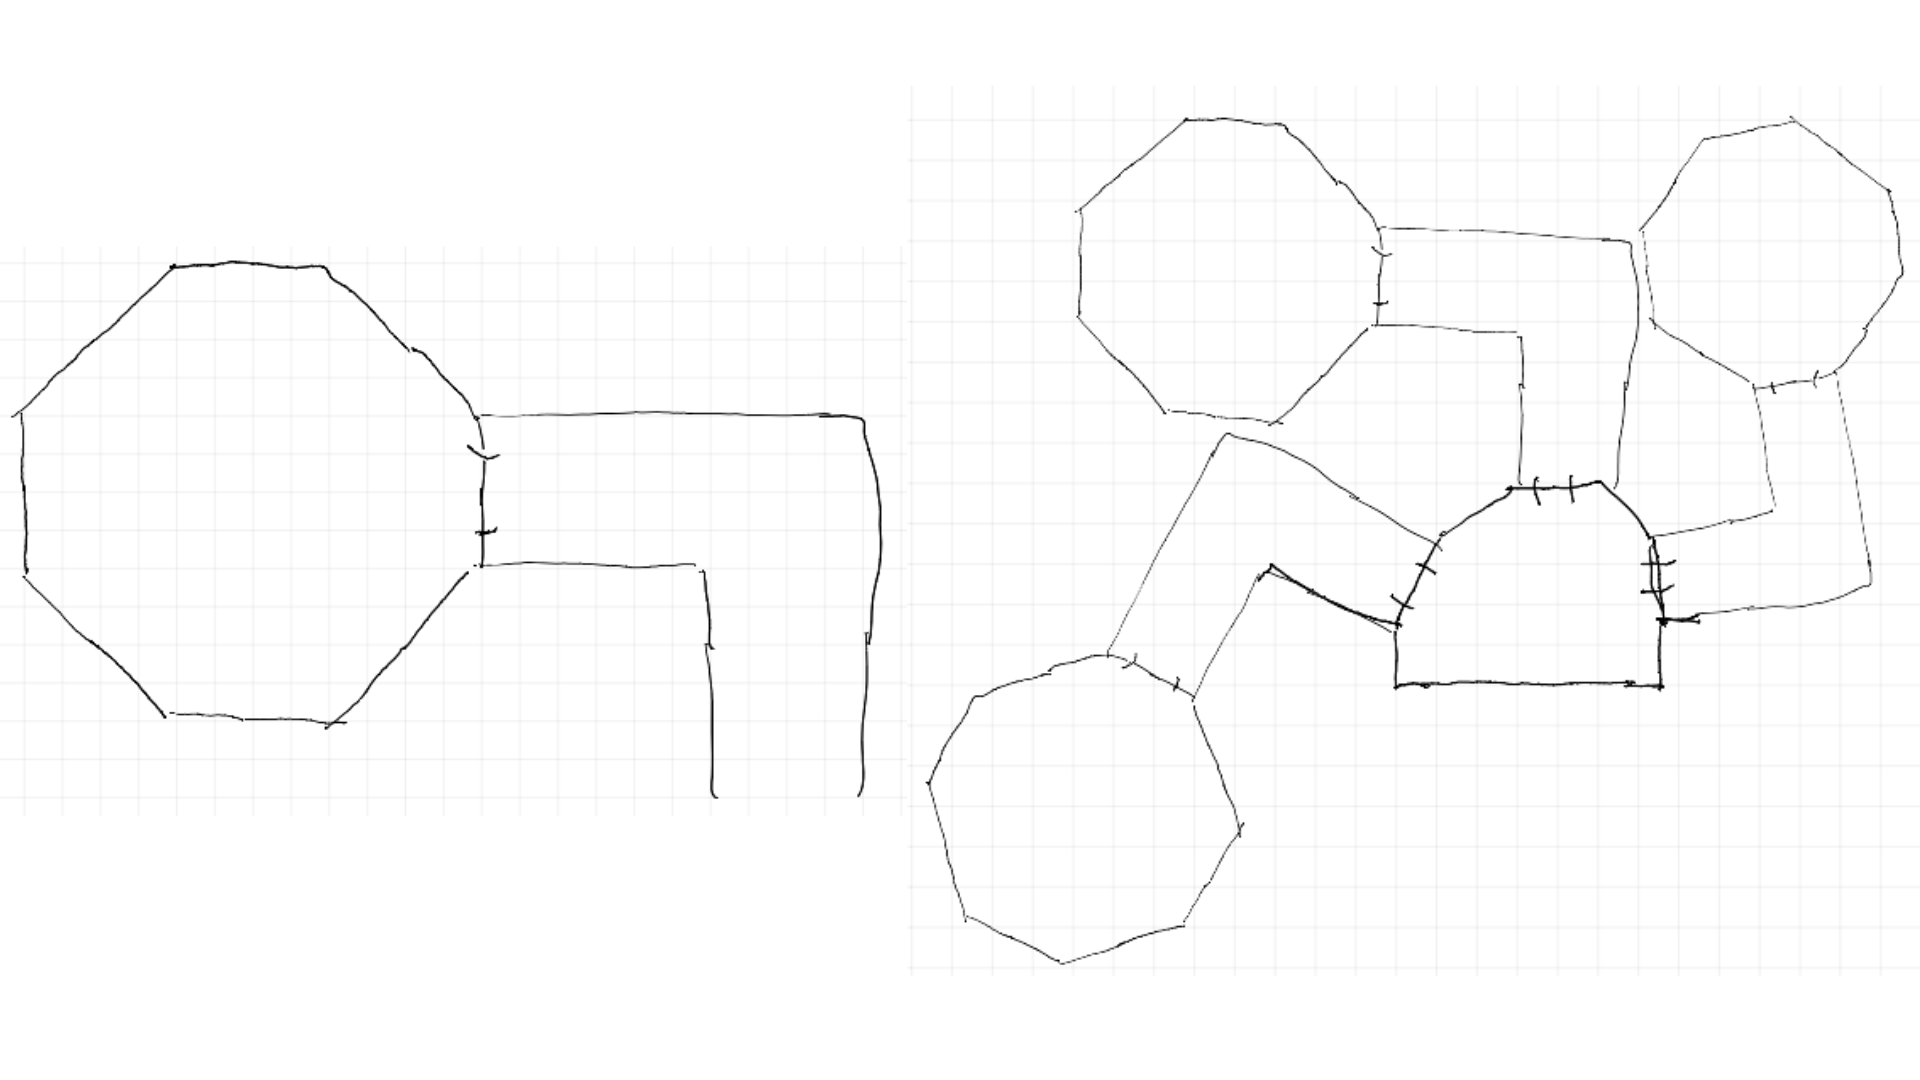
\includegraphics[width=1\linewidth]{content/pictures/Abschnitt_Concept_00.png}
\caption{Konzept Abschnitt 1 (Quelle: eigene Darstellung)}
\label{fig:section_00_concept}
\end{figure}

Abbildung \ref{fig:section_00_concept} zeigt eine erste Konzeptzeichnung des ersten Abschnittes. Sie beinhaltet links einen sechs-eckigen Raum, in dem der Spieler-Avatar des Players in die Spielwelt gesetzt wird. Diesen ersten Startraum gibt es, wie man auf der rechten Seite des Bildes sehen kann drei mal. Der Player muss seinem Watcher nun beschreiben in welchem der drei Räume er sich befindet. Die Räume unterscheiden sich dabei in ihrer Gestaltung. Wie in Abbildung \ref{fig:corridors} zu sehen, besitzt der erste Raum (erste Reihe, linkes Bild) einen Kronleuchter in der Mitte des Raumes, der zweite Raum (zweite Reihe, linkes Bild) einen großen Teppich und der dritte Raum (dritte Reihe, linkes Bild) eine Bank zwischen zwei Innensäulen.

\begin{figure}[ht]
\centering
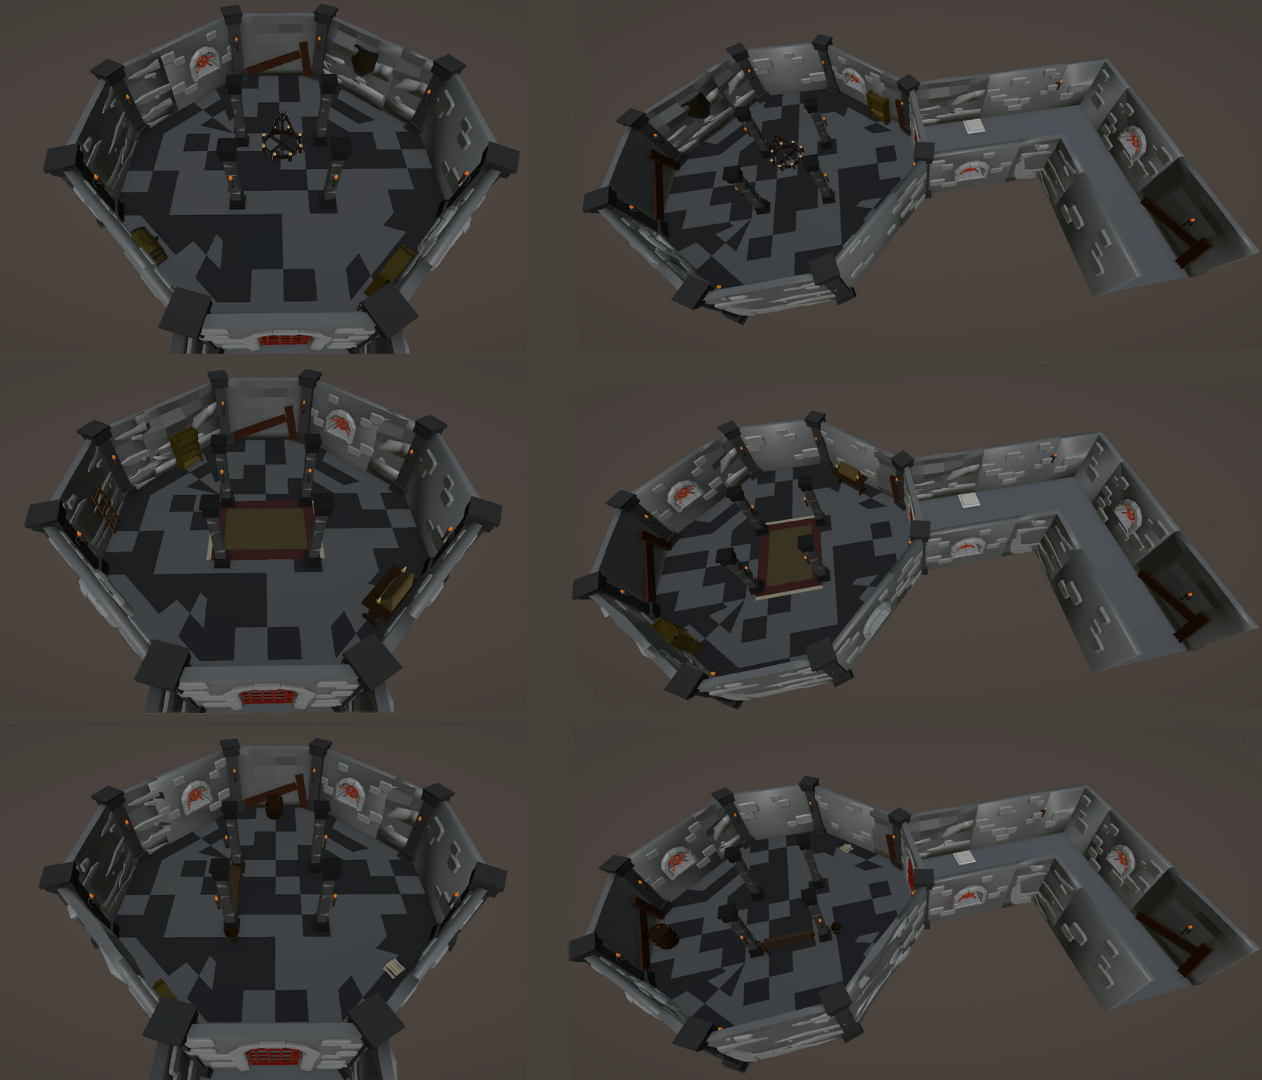
\includegraphics[width=1\linewidth]{content/pictures/Room_00-Room_02-Corridor_00-Corridor_02.png}
\caption{Korridor 1 bis Korridor 3 (Quelle: eigene Darstellung)}
\label{fig:corridors}
\end{figure}

Wie in der Konzeptzeichnung von Abbildung \ref{fig:section_00_concept} im rechten Bild zu sehen führen die Starträume über einen eckigen Flur in eine Eingangshalle. Dieser ist in Abbildung \ref{fig:section_00} zu sehen. An der entgegenfliegenden Wand von den drei eckigen Fluren aus ist eine Tür, durch die der Player mit Hilfe des Watchers gelangen muss um den folgenden Abschnitt freizuschalten. 

\begin{figure}[ht]
\centering
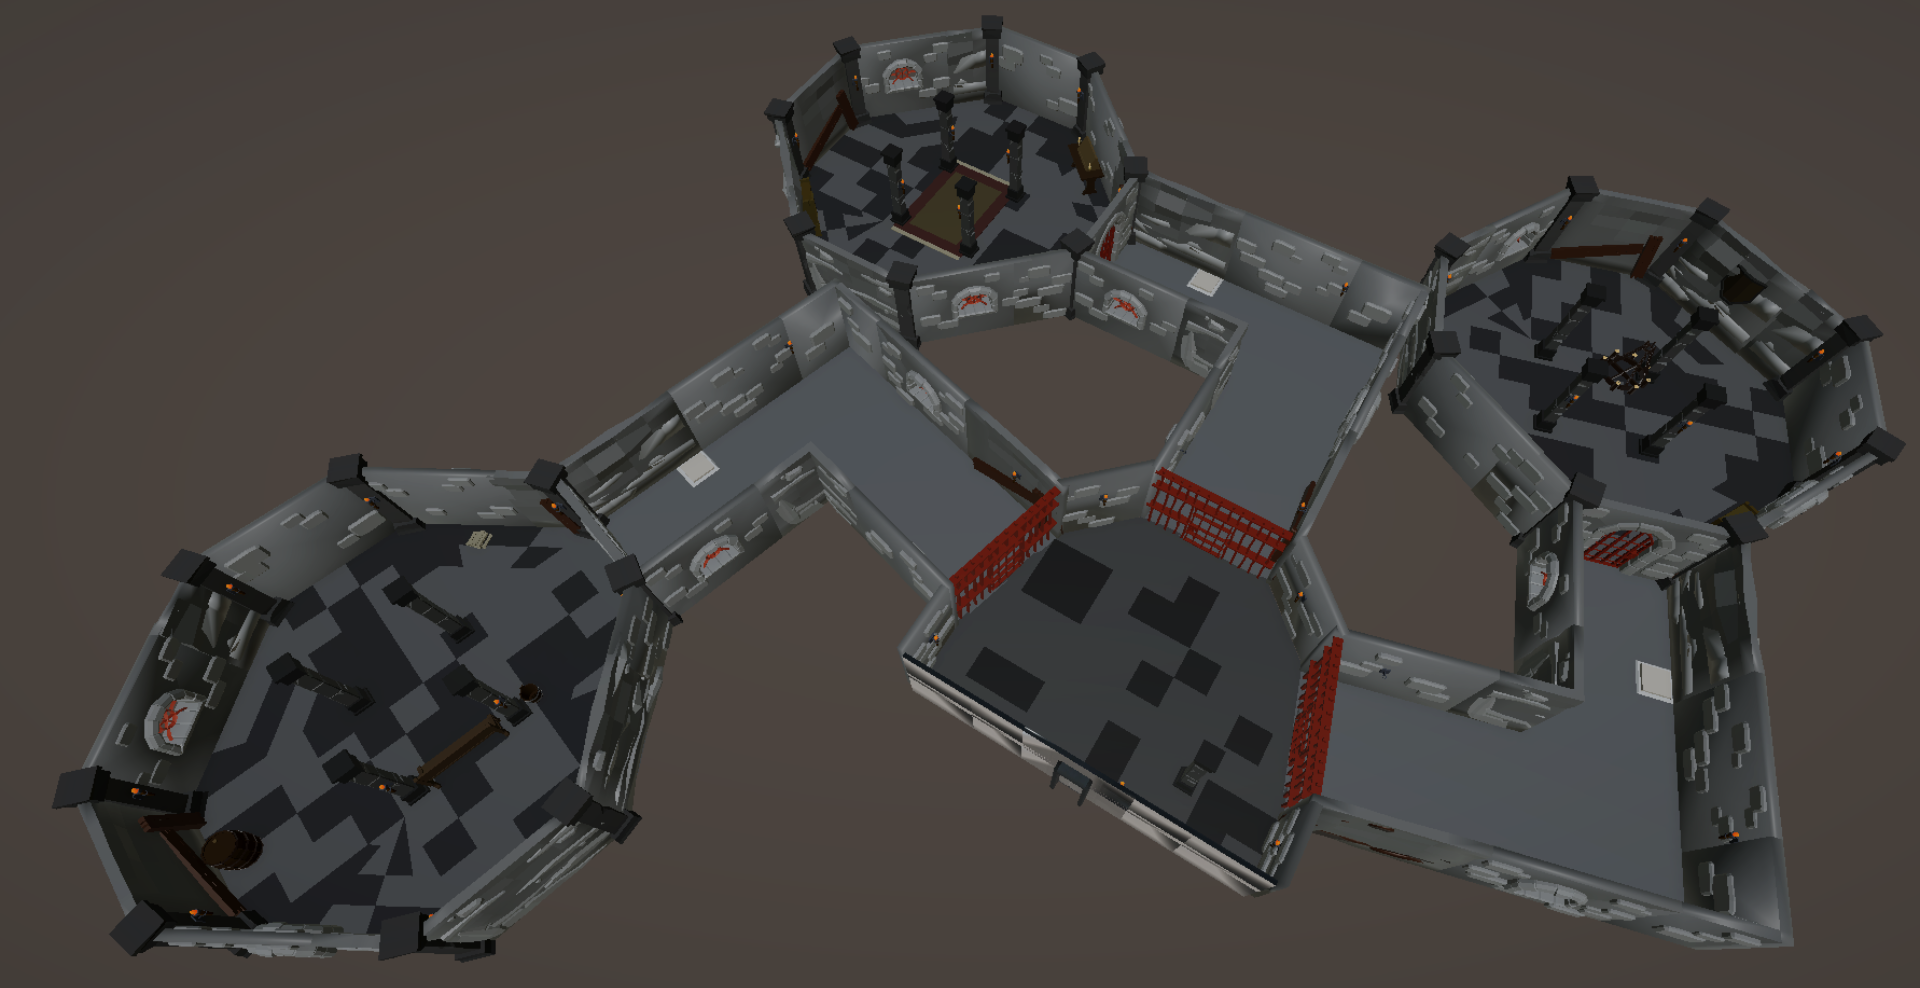
\includegraphics[width=1\linewidth]{content/pictures/Abschnitt_00.PNG}
\caption{Abschnitt 1 (Quelle: eigene Darstellung)}
\label{fig:section_00}
\end{figure}

Der Watcher sieht zum Start den gesamten ersten Abschnitt aus Abbildung \ref{fig:section_00}, wohingegen der Player nur einen der drei Starträume aus Abbildung \ref{fig:corridors} und den anliegenden Flur sehen kann. Die anderen zwei Räume samt Flur kann er nicht sehen. Auch dann nicht, wenn er in der Eingangskammer zum nächsten Abschnitt gelangt ist.

\paragraph{[Verschiedene Räume]}

\subsection{Rätsel}

\section{Dialoge}

\section{Sounddesign}



% \section{Rollenspezifisches Design}

% \section{Genre}

% \section{Spielmechanik}

% \section{Spielablauf}

% \subsection{Spielablauf des Spiels}

% \subsection{Levelablauf}

% \section{Session}

% % \section{Belohnungen}

% \section{Spielerrollen}

% \subsection{Player}

% % \subsubsection{Interaktion mit Gegenständen}

% % \subsubsection{Tragen von Gegenständen}

% \subsection{Watcher}

% % \subsubsection{Platzieren von Gegenständen}

% % \subsubsection{Entfernen von Gegenständen}

% % \subsubsection{Previewen von Gegenständen}

% \section{Gegenstände}

% \subsection{Leichte Gegenstände}

% \subsection{Schwere Gegenstände}

% \subsection{Hinweise}

% \section{Leveldesign}

% \subsection{Gegenstände}

% \subsection{Hinweise}

% \subsection{Hindernisse}

% \section{Informationen für den Spieler}

% \section{Sounddesign}

% \chapter{Visuelles Design des Prototyps}

% \section{Moodboard}

% \section{Art-Stil}

% \section{Avatar des Players}

% \section{User Interface}

% \section{Führung durch das Level}

% \section{Gegenstände}

% \section{Menü}

% \section{Leveldesign}